%%%%%%%%%%%%%%%%%%%%%%%%%%%%%%%%%%%%%%%%%%%%%%%%%%%%
% This will help you in writing your homebook
% Remember that the character % is a comment in latex
%
% chapter 1
\chapter{More in details}
\label{chap1}

\section{ALU}

The core of all operations is the ALU, collocated in the execution unit. It is the component in charge of doing logical
and arithmetical operations. The ALU is configured externally by the C.U., selecting which is the function.
\\It is composed of :

\begin{itemize}
\item Adder;
\item Multiplier;
\item Logic;
\item Comparator;
\end{itemize}

\subsection{Adder}

The architecture of our adder is like the P4 one implemented during laboratories. We choose this configuration to avoid high carry
delays and to make the sum faster. The general architecture is:

\begin{figure}[ht]
\centering
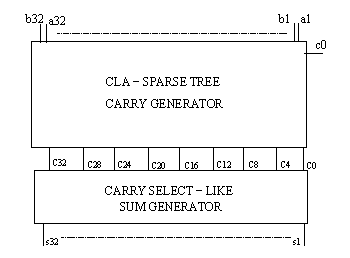
\includegraphics[]{chapters/figures/p4adder} 
\caption{P4 Adder schematic.}
\label{fig:adder}  % here is the figure label
\end{figure}

The two blocks are in charge of doing a sum or a subtraction. The idea is to compute partial carries and propagate them into the sum 
generator, reducing the computational time w.r.t. the traditional Ripple Carry Adder. Obviously, to obtain the configuration for the subtraction,
the second input B is xored with Cin.\\
\paragraph{Carry generator}
The sparse tree carry generator architecture is shown below:

\begin{figure}[h]
\centering
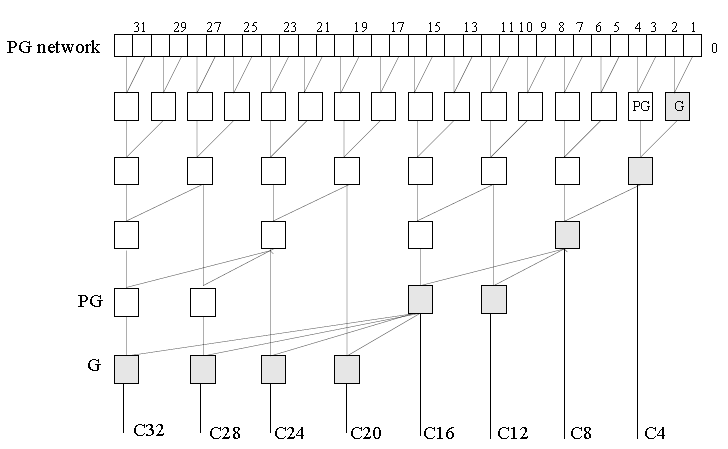
\includegraphics[scale = 0.3]{chapters/figures/sparsetree} 
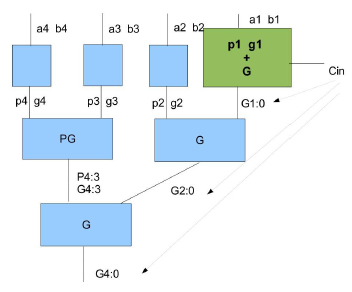
\includegraphics[scale = 0.5]{chapters/figures/sparsetreedetails} 
\caption{P4 Adder Carry generator and details.}
\label{fig:sparsetree}  % here is the figure label
\end{figure}

G and PG blocks implement general Generate and Propagate blocks, defined as:

\begin{align}
	G_{i:j} &= G_{i:k} + P_{i:k} * G_{k-1:j};\\
	P_{i:j} &= P_{i:k} * P_{k-1:j};
\label{General P and G}
\end{align}
	
where

\begin{itemize}
\item  i $\ge$ k $>$ j;
\item G$_{x:x}$ = g$_{x}$ that is the generate term and P$_{x:x}$ = p$_{x}$ that is the propagate term;
\item g$_{0}$ = Cin and p$_{0}$ = 0;
\item g$_{i}$ = a$_{i}$ * b$_{i}$;
\item p$_{i}$ = a$_{i}$ + b$_{i}$;
\end{itemize}

\begin{figure}[h]
\centering
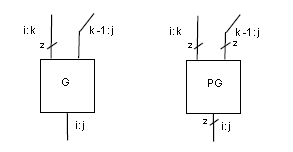
\includegraphics[scale = 0.5]{chapters/figures/ppgblocks} 
\caption{Block G and PG.}
\label{fig:gpgblocks}  % here is the figure label
\end{figure}

The first G$-$block generate only G$_{i:j}$ and the other PG$-$block generate both G$_{i:j}$ and P$_{i:j}$.

\paragraph{Sum Generator}

This block is a Carry$-$Select Adder, each subblock use a Ripple Carry Adder for partial sums. 

\begin{figure}[h]
\centering
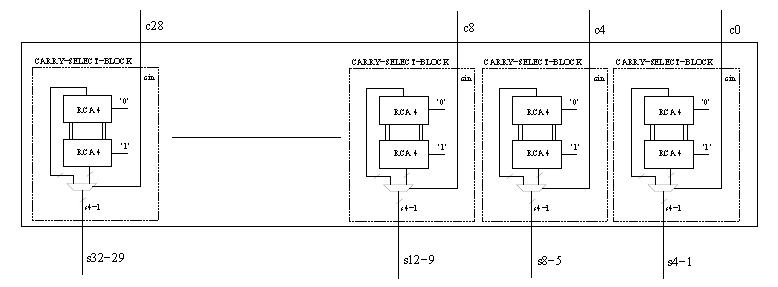
\includegraphics[scale = 0.7]{chapters/figures/sumgen} 
\caption{Carry Select Adder with Carries coming from sparse tree.}
\label{fig:sumgen}  % here is the figure label
\end{figure}

\begin{figure}[h]
\centering
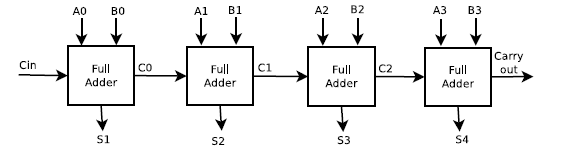
\includegraphics[scale = 0.7]{chapters/figures/rca} 
\caption{4-bit RCA inside p4 adder.}
\label{fig:rca}  % here is the figure label
\end{figure}

\FloatBarrier

\subsection{Multiplier}



\subsection{Logic}

We implement a simple way to do logic operations. The operands pass through 32 parallel gates bit by bit, implementing the requested operation. 
We choose this configuration in order to have the same delay for all bits of operands, even if it results in a large area.
\\Examples: 
\begin{itemize}
\item ALUOut$_{i}$ $<=$ A$_{i}$ and B$_{i}$;
\item ALUOut$_{i}$ $<=$ A$_{i}$ or B$_{i}$;
\end{itemize}

\subsection{Comparator}

We use the comparator for conditional instructions. We choose to implement a classic architecture, using an adder in
subtraction configuration and gates. The architecture is the following:

\begin{figure}[!h]
\centering
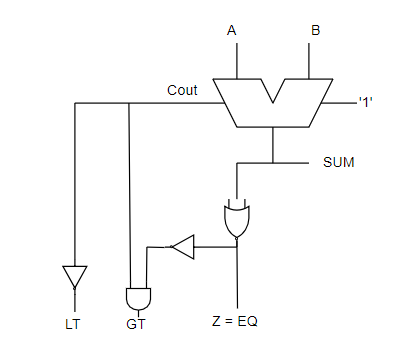
\includegraphics[scale = 0.7]{chapters/figures/comparator} 
\caption{Comparator.}
\label{fig:comparator}  % here is the figure label
\end{figure}

\FloatBarrier

Then we implement a process which verifies if the input condition from the C.U. is satisfied or not, and send a signal Taken in output. 
(Taken = '1' means satisfied and viceversa, See Appendix B for VHDL code).





 